
\section{All combined limits}
\label{results}

Figure~\ref{fig:HVCombined} shows the limits for combining $\Hbb$ and $\Hww$ decaying channels together in 
the five categories. The Higgs and V bosons branching ratios are already taken into account.  
In HVT B model, W' and Z' are degenerate, having about the same mass. So we also show the combined limit of 
W' and Z' here.  


\begin{figure}[ht!pb]
\begin{center}
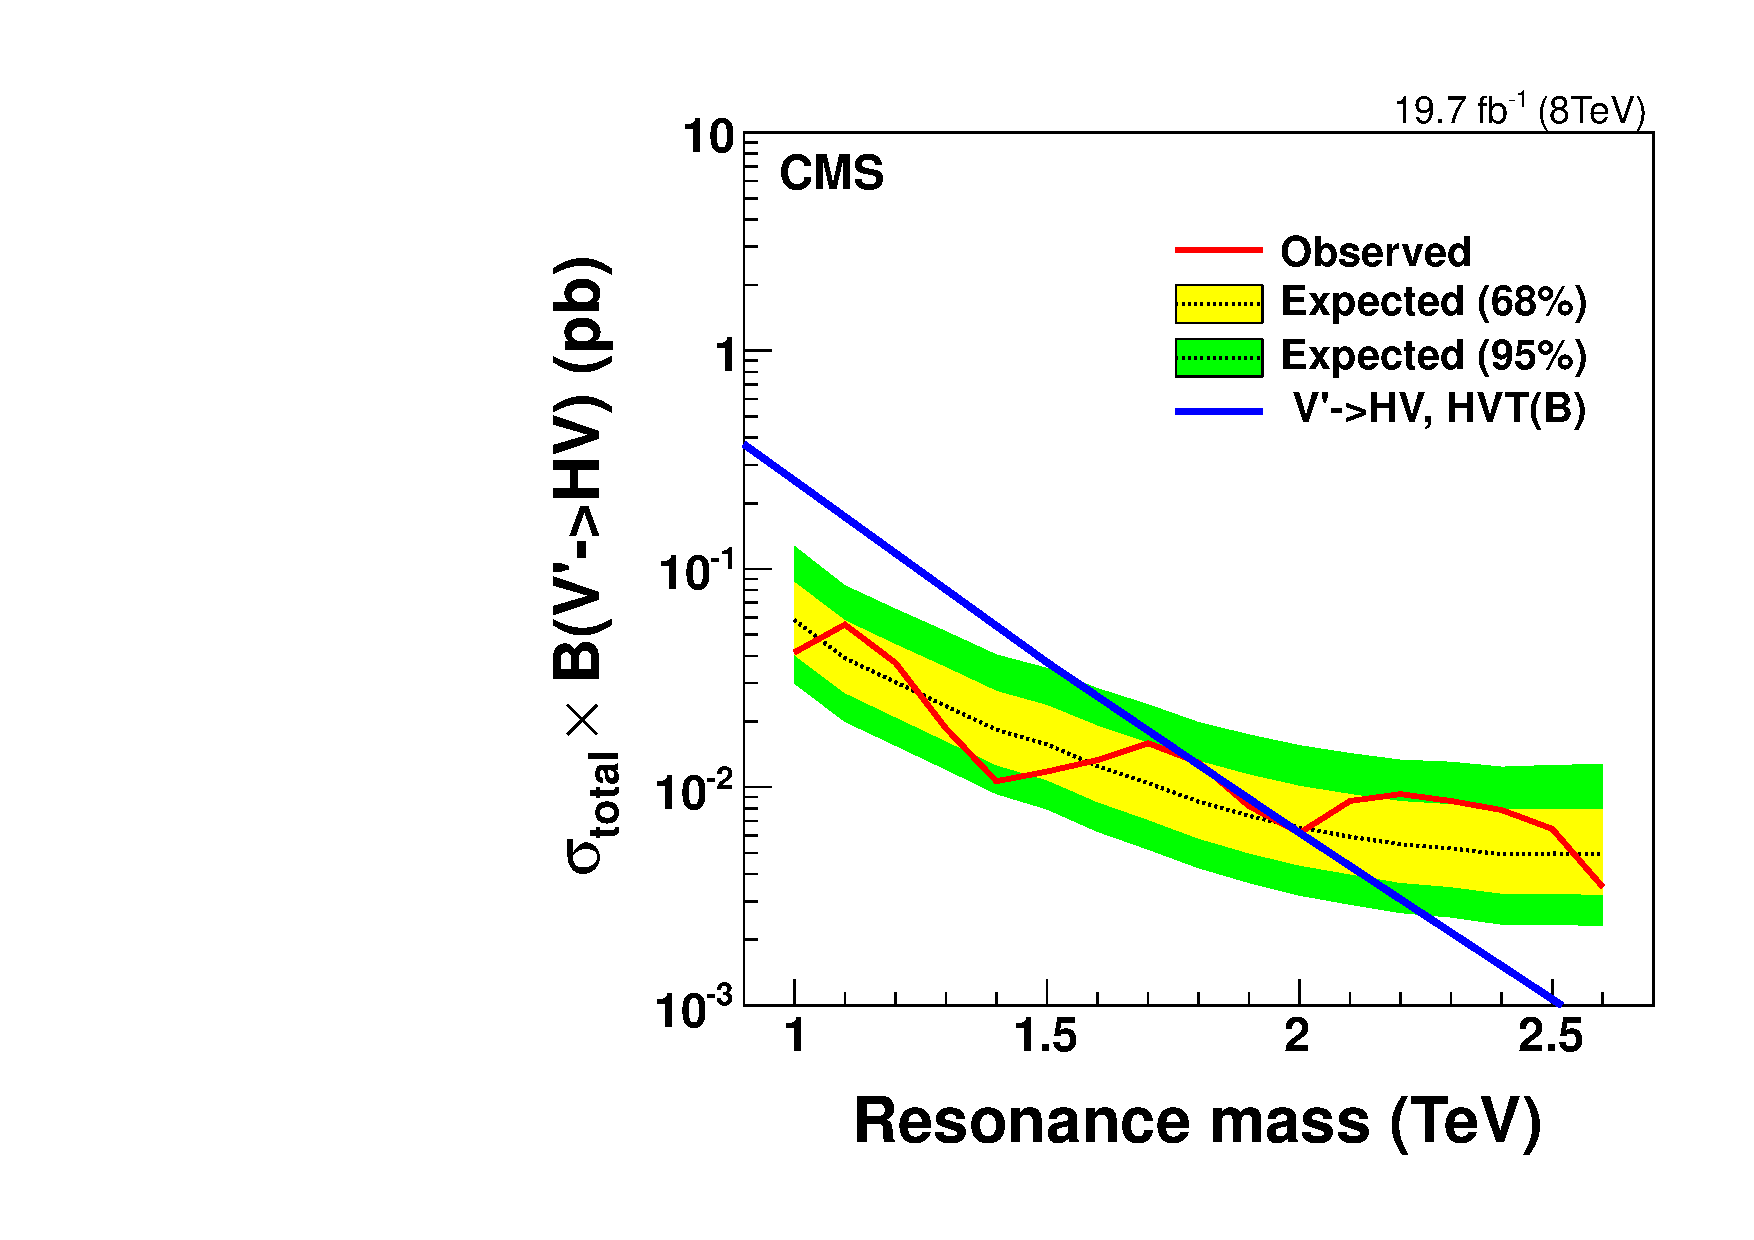
\includegraphics[width=0.7\textwidth]{EXO-14-009/brazilianFlag_HV.pdf}
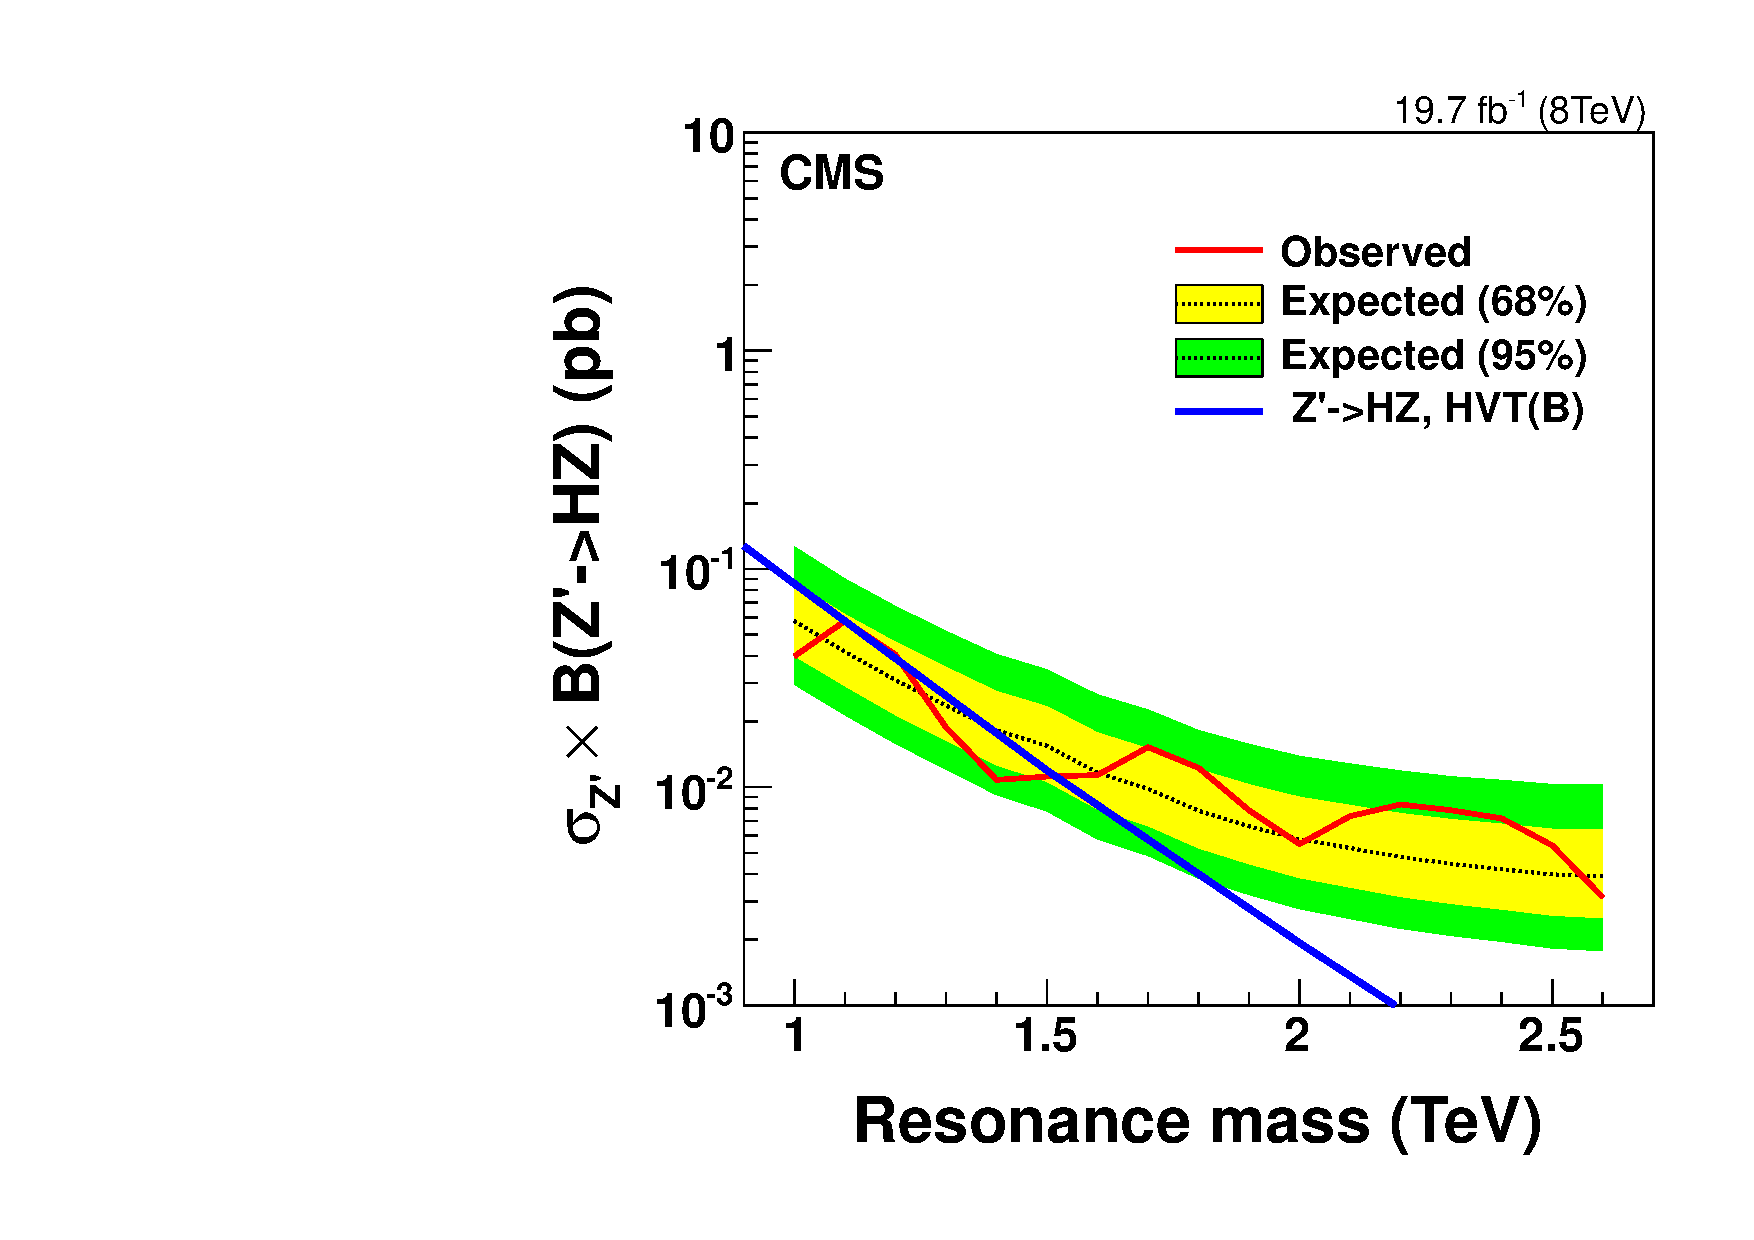
\includegraphics[width=0.49\textwidth]{EXO-14-009/brazilianFlag_HZqq.pdf}
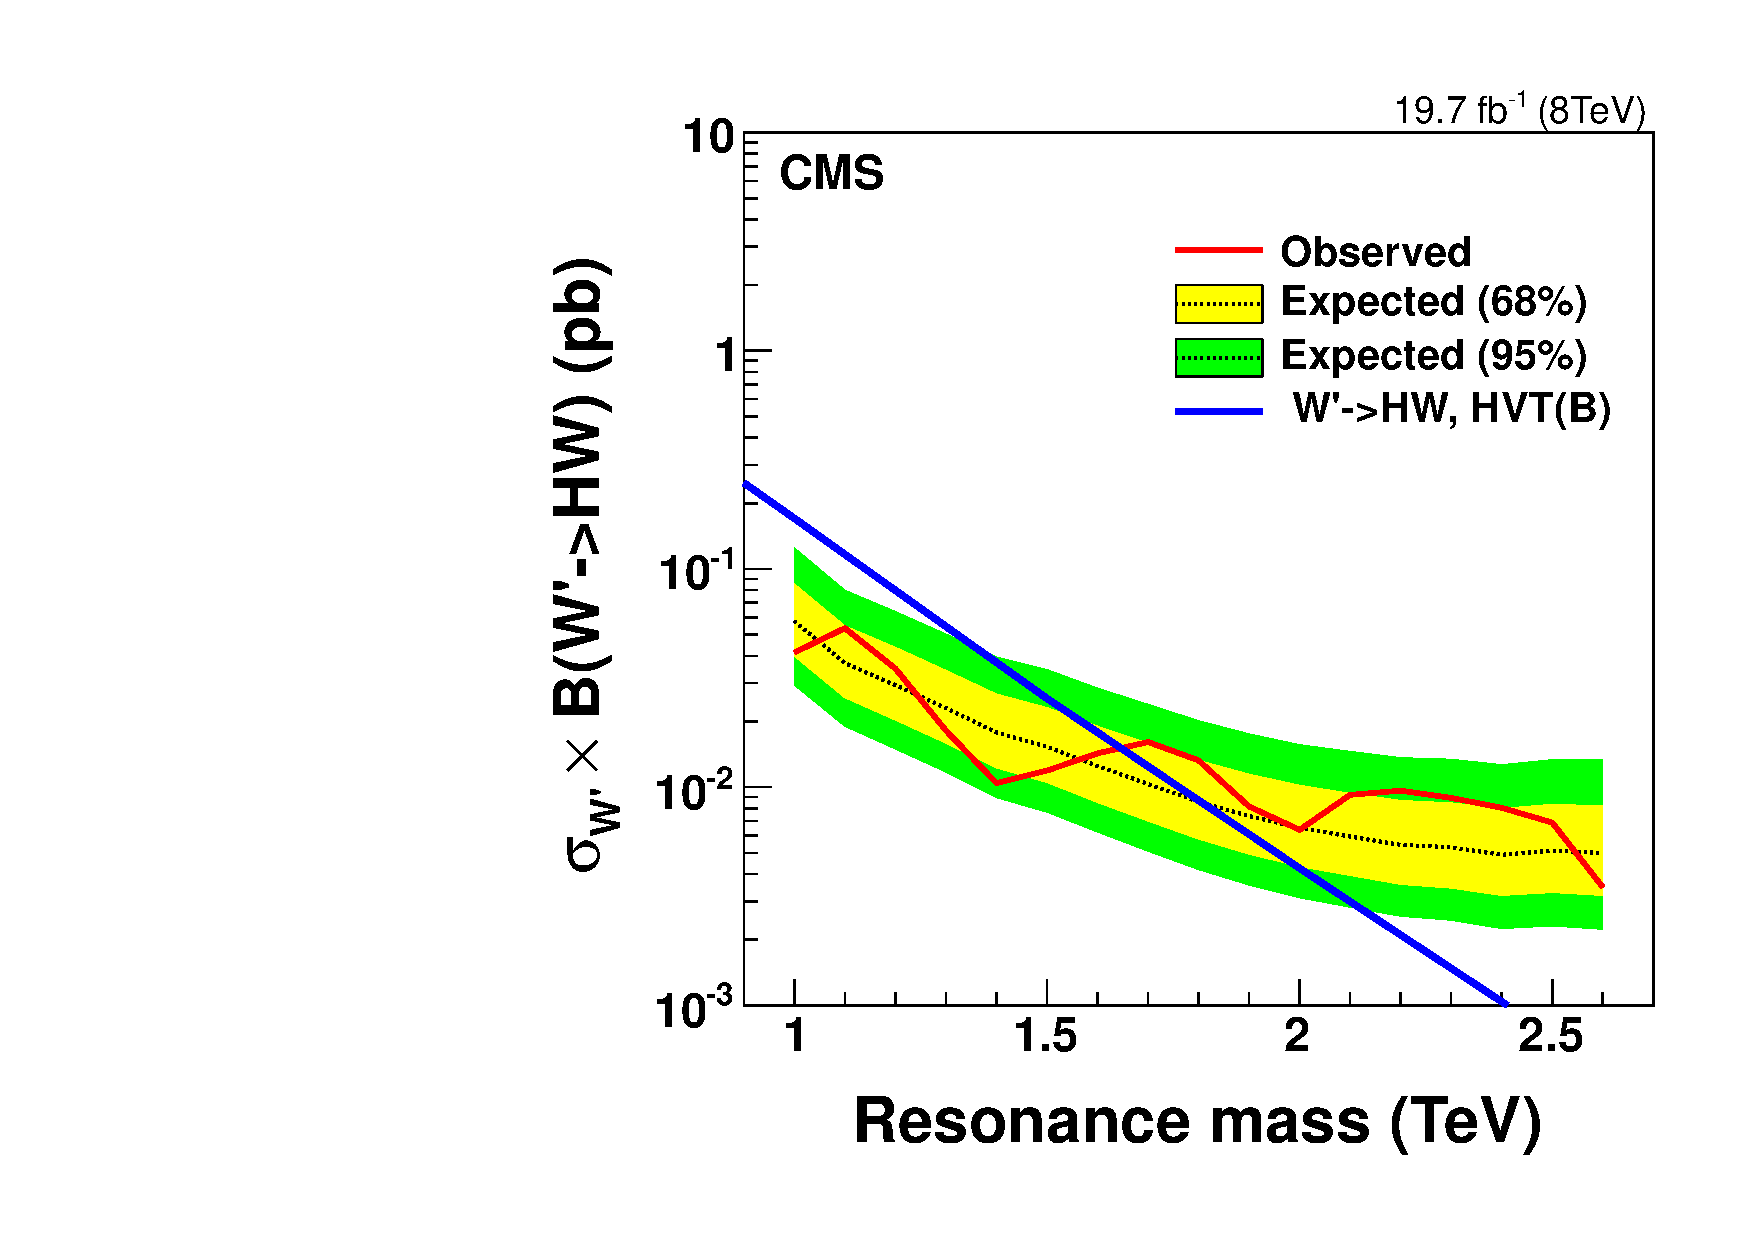
\includegraphics[width=0.49\textwidth]{EXO-14-009/brazilianFlag_HWqq.pdf}
\end{center}
\caption{W' and Z' combined limit is the top plot, by considering them having the same mass, including all the categories in this analysis.   
Combined expected and observed limits for ${\rm Z'\to HZ}$ (bottom left) and ${\rm W' \to WH}$ (bottom right),  including $\Hbb$ and $\Hww$ channels. Branching ratios of Higgs and V decays 
are already taken into account. Theory model used here is HVT scenario B, arXiv:1402.4431.  
% The high purity is on the bottom left. the low purity V-tagging on bottom right.
%  The predicted cross sections as a function of resonance mass for the considered benchmark models are overlaid.
}
\label{fig:HVCombined}
\end{figure}

